\subsection{Schätzverfahren}
\label{sec_curveFit}
In diesem Abschnitt wird das implementierte Schätzverfahren erläutert. Das Verfahren nutzt die Erkenntnisse der Bilderkennung und versucht mithilfe der Regression ein Polynom $f$ zweiten \todo{Welcher Grad} Grades durch alle erkannten Punkte in Betrachtung ihrer Orientierung zu fitten.
Das Verfahren basiert auf dem \textit{Least-Squares} Verfahren\cite{simon2006optimal}, wobei versucht wird die Gleichung [\ref{lsq}] zu minimieren.\\
$x_i$ und $y_i$ sind hierbei die Koordinaten der erkannten Punkte. Es wird über alle Punkte summiert der quadratische Fehler vom Funktionswert zu gegebenen Parametern zum $y$ aus der Bilderkennung berechnet. $f(p,x)$ ist eine beliebige Funktion, die $x$ in Abhängigkeit von $p$ auf eine reelle Zahl abbildet.\\
\begin{ownequation}[H]
\begin{equation}
err = \sum_{i}(f(p,x_i)-y_i)^2
\end{equation}
\caption{Least Squares Verfahren}
\label{lsq}
\end{ownequation}
Die Ergebnisse der Bildverarbeitung können nicht alle gleich behandelt werden. Faktoren wie Sichtbedingung, Helligkeit des Bildes oder auch die Sichtbarkeit/Bedeckung des Objektes beeinflussen die Güte eines erkannten Punktes. Ebenso beeinflussen die Neigungswinkel des AUVs die Güte der Transformation (\ref{section_PicToCam}), somit sind auch Punkte die bei hohen Neigungswinkeln detektiert wurden schlechter zu bewerten.\\
Neben den qualitativen Merkmalen eines Punktes ist es ebenso sinnvoll alte Punkte über die Zeit schlechter zu Bewerten. Für eine gute Verfolgung eines Objektes sollten die zuletzt erkannten Punkte weitaus wichtiger sein, als Punkte die bereits mehrere Meter entfernt liegen.
Um diese Anforderungen umzusetzen habe ich eine Erweiterung des \textit{Least-Squares} genutzt, den \textit{Weighted-Least-Squares}[\ref{wlsq}]\\
\begin{ownequation}[H]
\begin{equation}
err = \sum_{i}w_i \cdot (f(p,x_i)-y_i)^2
\end{equation}
\caption{Weighted Least Squares Verfahren}
\label{wlsq}
\end{ownequation}

Das \textit{Weighted-Least-Squares} Verfahren bietet eine gute Grundlage für die Regression. Es bleiben jedoch noch einige Probleme, die das Verfahren in der Form nicht lösen kann.
\begin{enumerate}
\item Beachtung der Orientierung erkannter Punkte
\item Bedingungen für die Kurve (z.B. maximale Steigung)
\item Schätzungen, für Punktverläufe, die sich nicht durch eine einzelne Funktion darstellen lassen
\end{enumerate}

Zum Lösen der ersten zwei Probleme bietet die \matlab Funktion \textit{fmincon} eine geeignete Lösung. Die Funktion bietet die die Möglichkeit eine Funktion $F(p)$ zu minimieren, wobei mit $c(p) \leq 0$ eine Bedingung erfüllt werden muss. Die Funktion $c(p,x_i)$ [\ref{constraint}] berechnet über den Funktionsverlauf von $f(p,x)$ mithilfe der Ableitung $f'(p,x)$ die Steigung in jedem Punkt $x_i$. Da \textit{fmincon} prüft, ob die Bedingungsfunktion kleiner 0 ist wird von der Steigung ein Maximalwert ($max_{slope}$) abgezogen (\textit{Erfüllt 2.}).\\
\begin{ownequation}[H]
\begin{equation}
c(p,x_i) = f'(p,x_i)-max_{slope}
\end{equation}
\caption{Funktion zum überprüfen, ob die Steigung einen Maximalwert nicht übersteigt.}
\label{constraint}
\end{ownequation}
Die Funktion $F(p)$ wird als $F(p,x,y,s,w,n,m,tau)$ [\ref{minimizeFunction}] definiert, wobei $x$ und $y$ wieder die Punkte der Bilderkennung darstellen, $s$ die erkannte Orientierung im Punkt und $w$ das Gewicht der Punkte. Die Funktion $F$ besteht aus einer Linearkombination der Funktionen $g$ und $h$, wobei $g$ den summierten Fehler der Position [\ref{posError}] ($x$,$y$ Koordinaten) und $h$ den summierten Fehler der Orientierung [\ref{orienError}] mithilfe des \textit{Weighted-Least-Squares} Verfahren berechnen (\textit{Erfüllt 1.}). $n$ und $m$ Gewichten, wie stark die einzelnen Fehlerarten (Position und Orientierung) in den Gesamtfehler für die gegebenen Funktionsparameter $p$ beeinflussen.\\
Um die erhaltene Polynome einschränken zu können wurde $F$ noch gemäß der \textit{Tikhonov Regularisierung} \cite{kaipio2006statistical} angepasst. Durch die \textit{Tikhonov Regularisierung} können wenig gekrümmte Kurven bevorzugt werden, was für einen ruhigeren Fahrtverlauf sorgen kann.
\begin{ownequation}[H]
\begin{equation}
\label{minimizeFunction}
F(p) = F(p,x,y,s,w,n,m,tau) = n \cdot g(p,x,y,w) + m \cdot h(p,x,s,w) + tau \cdot p
\end{equation}
\begin{equation}
\label{posError}
g(p,x,y,w) = \sum_{i} w_i \cdot (f(p,x_i)-y_i)^2
\end{equation}
\begin{equation}
\label{orienError}
h(p,x,s,w) = \sum_{i} w_i \cdot (f'(p,x_i)-s_i)^2
\end{equation}
\caption{Zusammensetzung der Funktion F, die minimiert wird.}
\label{F-function}
\end{ownequation}
\todo{neute Grafiken auch mit Translation}
Um das Problem 3. zu lösen betrachten wir Abbildung \ref{prob3}. Hierbei sind die erkannten Punkte so angeordnet, dass keine Funktion $f(x)$ gefunden werden kann, um die Punkte sinnvoll zu verbinden. Zum einen laufen die Punkte teilweise parallel zur $Y-Achse$ (in diesem Fall müsste die Steigung unendlich groß sein) und zum anderen gibt es Werte $y_1 \neq y_2$, sodass gelten müsste $y_1 = f(x_n) = y_2$ für ein bestimmtes $n$. Dies verstößt jedoch gegen die Definition einer Polynomialfunktion.\\
\begin{figure}[H]
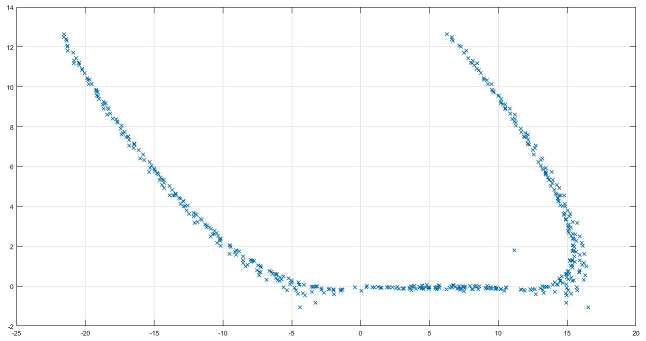
\includegraphics[scale=0.45]{curveFitting/pointsProblem.jpg}
\caption{Problem 3 vom Curve Fitting}
\label{prob3}
\end{figure}
In Abbildung \ref{prob3Marked} sind zwei Bereiche gekennzeichnet. Über den Bereich im schwarzen Kasten lässt sich noch gut eine Kurve legen (\ref{prob3Marked_a}). Kommt jedoch der Rote Bereich dazu würde eine Kurve über alle Punkte die Daten nicht mehr richtig abbilden.

\begin{figure}
\begin{tabular}{l}
\subfloat[Gesamter Datensatz in Bereiche unterteilt.]{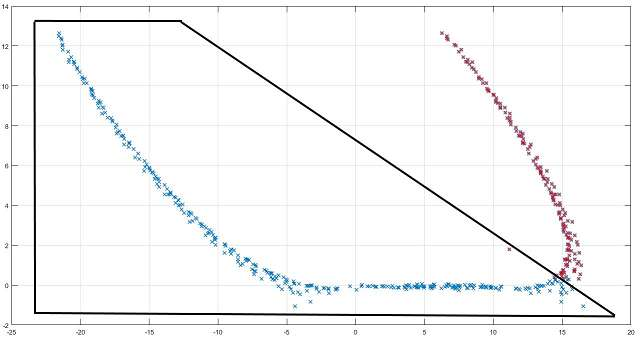
\includegraphics[scale=0.45]{curveFitting/pointsProblemMarks.jpg}\label{prob3Marked_a}}\\
\subfloat[Kurve durch den blauen Bereich. Die Kurve lässt sich nicht im roten Bereich fortführen.]{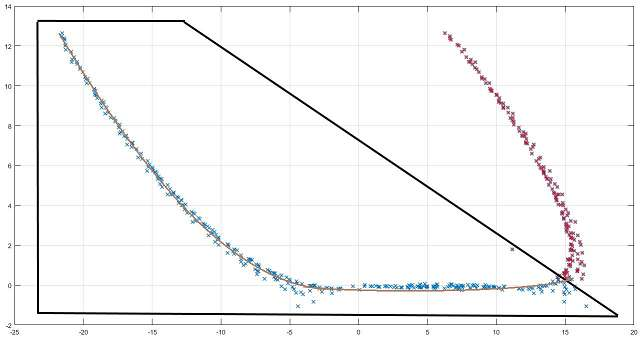
\includegraphics[scale=0.45]{curveFitting/pointsProblemMarksWithCurve.jpg}\label{prob3Marked_b}}
\end{tabular}
\caption{Detektionsdaten in Bereiche unterteilt.}
\label{prob3Marked}
\end{figure}

Um dieses Problem zu lösen werden die Punkte in Teilbereiche unterteilt (siehe \ref{solve3}). Mit jedem neu von der Bilderkennung erhaltenen Punkt wird eine neue Kurve mit dem beschriebenen Verfahren berechnet. Die so entstandene Kurve wird dann mithilfe der neuesten Punkte geprüft. Sollte der Fehler in diesen Punkten einen Schwellwert überschreiten gilt der Bereich als abgeschlossen und ein neuer Bereich wird begonnen. Dieser neue Bereich zeichnet sich durch eine Rotation der $X-Achse$ um den Wert der Ableitung der letzten Funktion $f'(x_m)$ an der letzten Stelle $x_m$ aus.\\
Neben der Rotation wird der neue Bereich noch so verschoben, dass der transformierte Koordinatenursprung im letzten erkannten Punkt liegt. Diese Maßnahme ist nötig, um die Punkte stets in auf möglichst nah am Koordinatenursprung zu halten. Betrachtet man die Geraden in \todo{grafik}, die sich nur durch ihre Verschiebung auf der $X-Achse$ unterscheiden und versucht Polynome zweiten Grades durch diese Graden zu legen gibt es für jede Gerade zwei mögliche Formen der Polynome. Auch diese Polynome ähneln sich in ihrer Geometrie sehr, jedoch sind die Parameter sehr unterschiedlich. Vor allem der Schnittpunkt zur $Y-Achse$ liegt bei der verschobenen Gerade sehr weit auseinander. Daraus resultiert, dass je weiter der aktuell abzufahrende Kurvenabschnitt vom Koordinatenursprung entfernt liegt, der Parameterraum für gute Polynome wächst. Dadurch steigt die Wahrscheinlichkeit für die Minimierungsfunktion in ein lokales Minimum zu laufen und nicht mehr auf sich ändernde Verläufe reagieren zu können.

\begin{tikzpicture}[domain=0:20]
    \draw[very thin,color=gray] (-0.1,-1.1) grid (3.9,3.9);
    \draw[->] (-0.2,0) -- (4.2,0) node[right] {$x$};
    \draw[->] (0,-1.2) -- (0,4.2) node[above] {$f(x)$};
    \draw[color=red, domain=0:5] plot(\x,\x); 
    \draw[color=red, domain=3:8] plot(\x,\x+5); 
\end{tikzpicture}


In [\ref{solve3}] sind die Teilbereiche der Punkte und die Punkte in ihrem jeweiligen rotierten Koordinatensystem angegeben.\\

\begin{figure}
\begin{tabular}{l}
\subfloat[Rotierter Datensatz im neuen Koordinatensystem (schwarz). Grün gestrichelt ist das ursprüngliche Koordinatensystem angedeutet.]{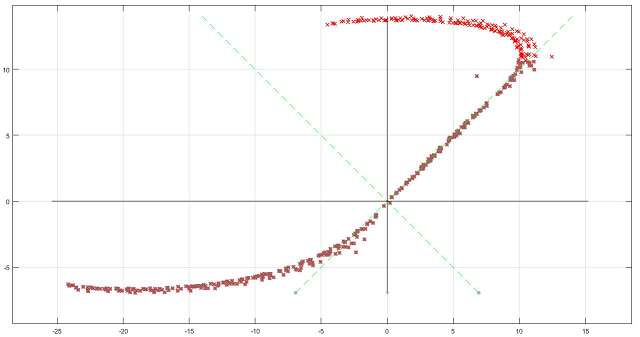
\includegraphics[scale=0.45]{curveFitting/pointsProblemSolved.jpg}\label{solve3Marked_a}}\\
\subfloat[Zwei Kurven durch den kompletten Datensatz. Die grüne Kurve entspricht der Kurve aus \ref{prob3Marked_b}. Die blaue Kurveaus dem rotierten Koordinantensystem.]{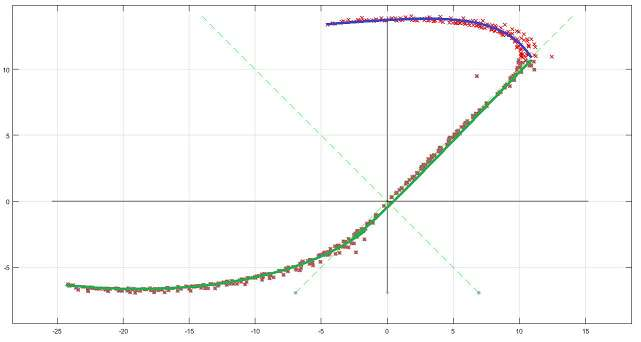
\includegraphics[scale=0.45]{curveFitting/pointsProblemSolvedWithCurves.jpg}\label{solve3Marked_b}}
\end{tabular}
\caption{Lösungsansatz für Problem 3 zum Curve Fitting}
\label{prob3solvedMarked}
\end{figure}

Zum Rotieren der Punkte werden beim Erzeugen eines neuen Bereichs die Rotationsmatrix $actual\_rotation$, sowie die Inverse $actual\_rotation\_inv$ berechnet und Zwischengespeichert. Sollte es bereits eine Rotation geben wird die neue Rotation durch Multiplikation der alten Rotation mit der neuen erzeugt.\\
Sobald eine Transformation vorhanden ist werden alle Punkte vor der Regression in das rotierte Koordinatensystem transformiert. Durch dieses Verfahren kann stets eine Kurve entlang der $X-Achse$ berechnet werden.

\subsubsection*{Generierung der Gewichte}
\label{sec_calcWeights}
In der Gleichung [\ref{F-function}] werden die Gewichte zur Berechnung des Fehlers genutzt. Im Vektor \textit{w} befindet sich genau ein Gewicht für jeden Punkt. Dieses setzt sich zum einen aus den Merkmalen der Objekterkennung [\ref{sec_weights}] und zum Anderen aus der Höhe des AUVs und den Neigungswinkeln zusammen.\\
In der Gleichung [\ref{weightsEquation}] ist die Berechnung des Gewichts für einen Punkt abgebildet. Alle Faktoren für das Gewicht werden als Linearkombination mit den Vorfaktoren $g_1$ bis $g_8$ zusammengefasst. Die Vorfaktoren werden mithilfe von Testdaten gelernt. Hierfür werden Objekte mithilfe von Funktionen in die Simulationsumgebung gelegt. Das AUV wurde dann mithilfe der gleichen Funktionen am Objekt entlang gesteuert. Die erkannten Punkte der Objekterkennung, sowie die Pose des AUVs wurden dabei aufgezeichnet.\\
Für jeder dieser Testdaten wird dann die Funktion $F$ [\ref{F-function}] optimiert. Der Unterschied hierbei ist jedoch, dass aufgrund der Definition des Objektes anhand von Funktionen die Funktionsparameter $p$ bekannt sind. Somit wird $F$ nicht mehr über die Parameter, sondern über die Vorfaktoren der Gewichte $g$ optimiert. Die so gelernten Faktoren werden dann in den Livebetrieb übernommen.
\begin{ownequation}[H]
\begin{equation}
\begin{split}
w &= g_1 \cdot numParts \\
&+ g_2 \cdot area \\
&+ g_3 \cdot peakheight \\
&+ g_4 \cdot fitsBorder \\
&+ g_5 \cdot relativeCount \\
&+ g_6 \cdot auvheight \\
&+ g_7 \cdot roll \\
&+ g_8 \cdot yaw
\end{split}
\end{equation}
\caption{Zusammensetzung des Gewichts für einen Punkt.}
\label{weightsEquation}
\end{ownequation}